
\section{tracert}

\subsection{Скриншоты}

\begin{center}

    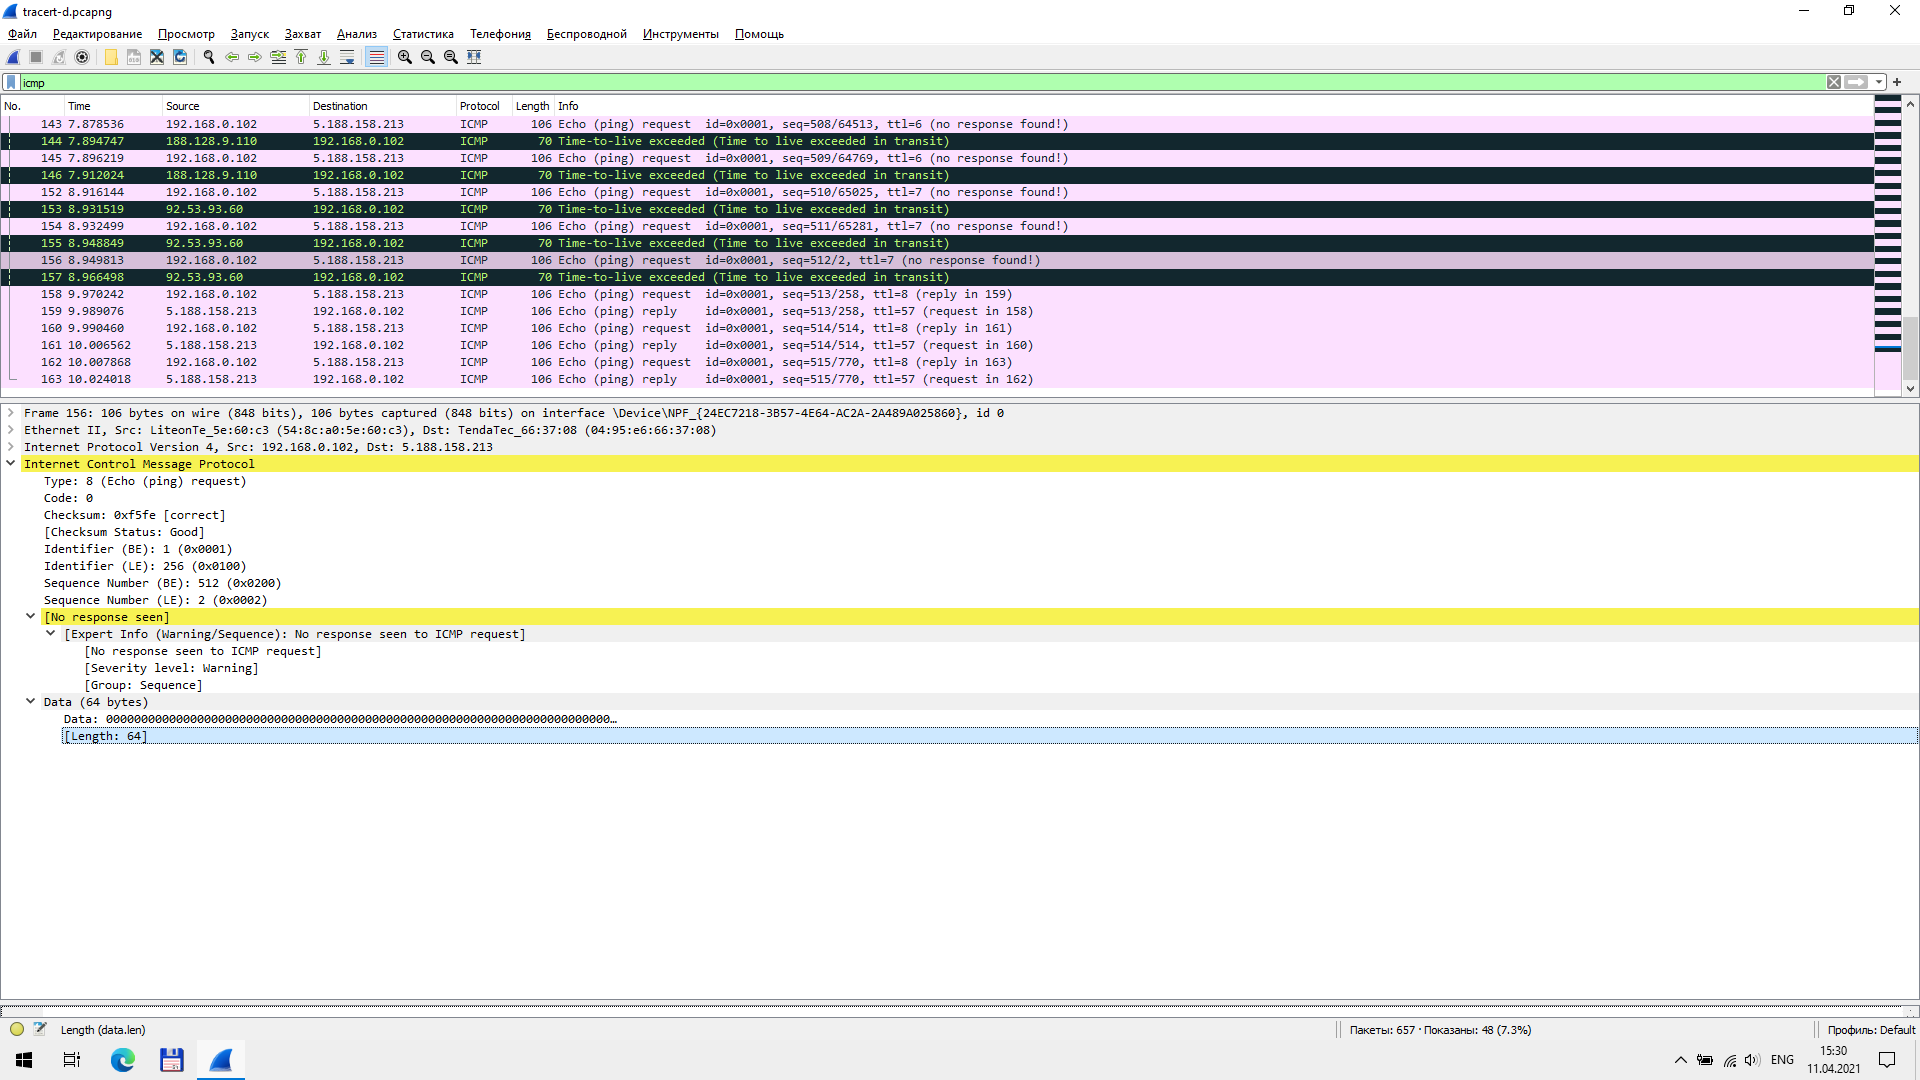
\includegraphics[width=\textwidth]{screenshots/tracert-d_ttl_request_1}

    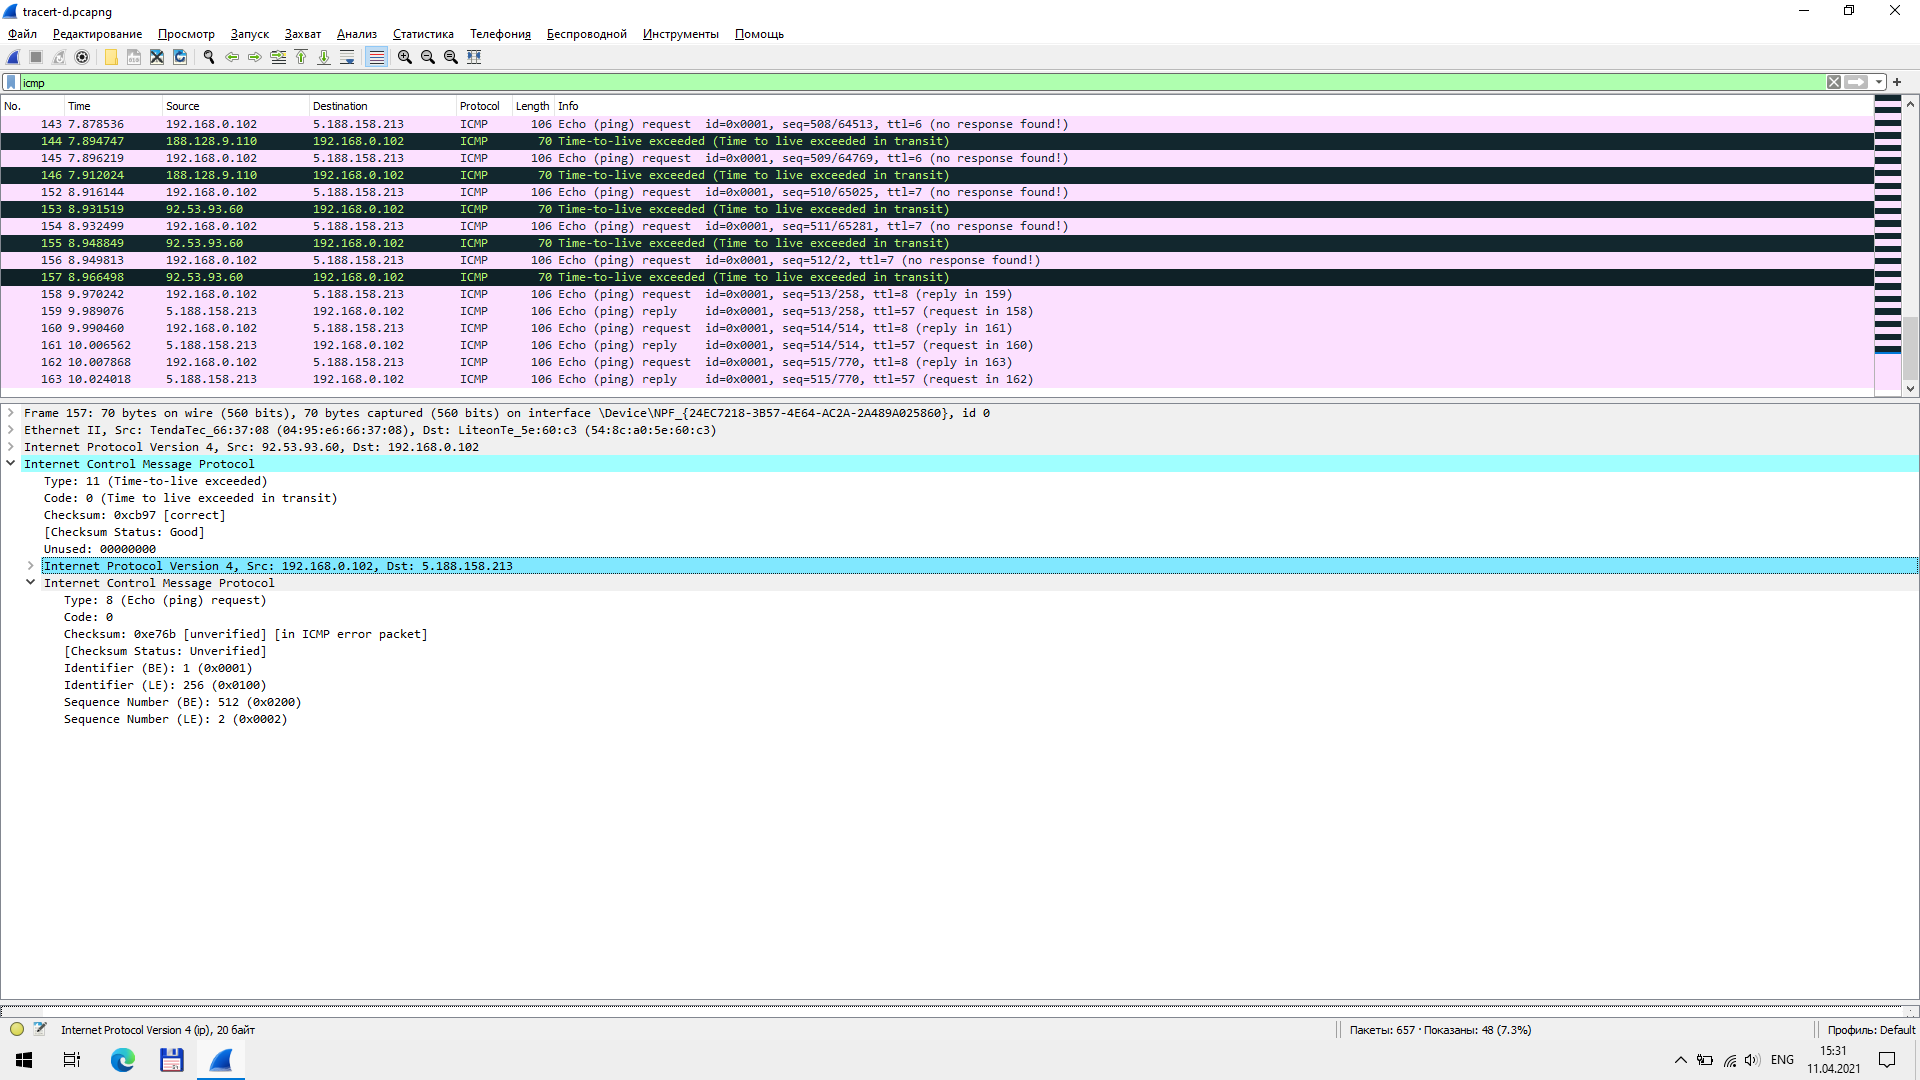
\includegraphics[width=\textwidth]{screenshots/tracert-d_ttl_response_1}

    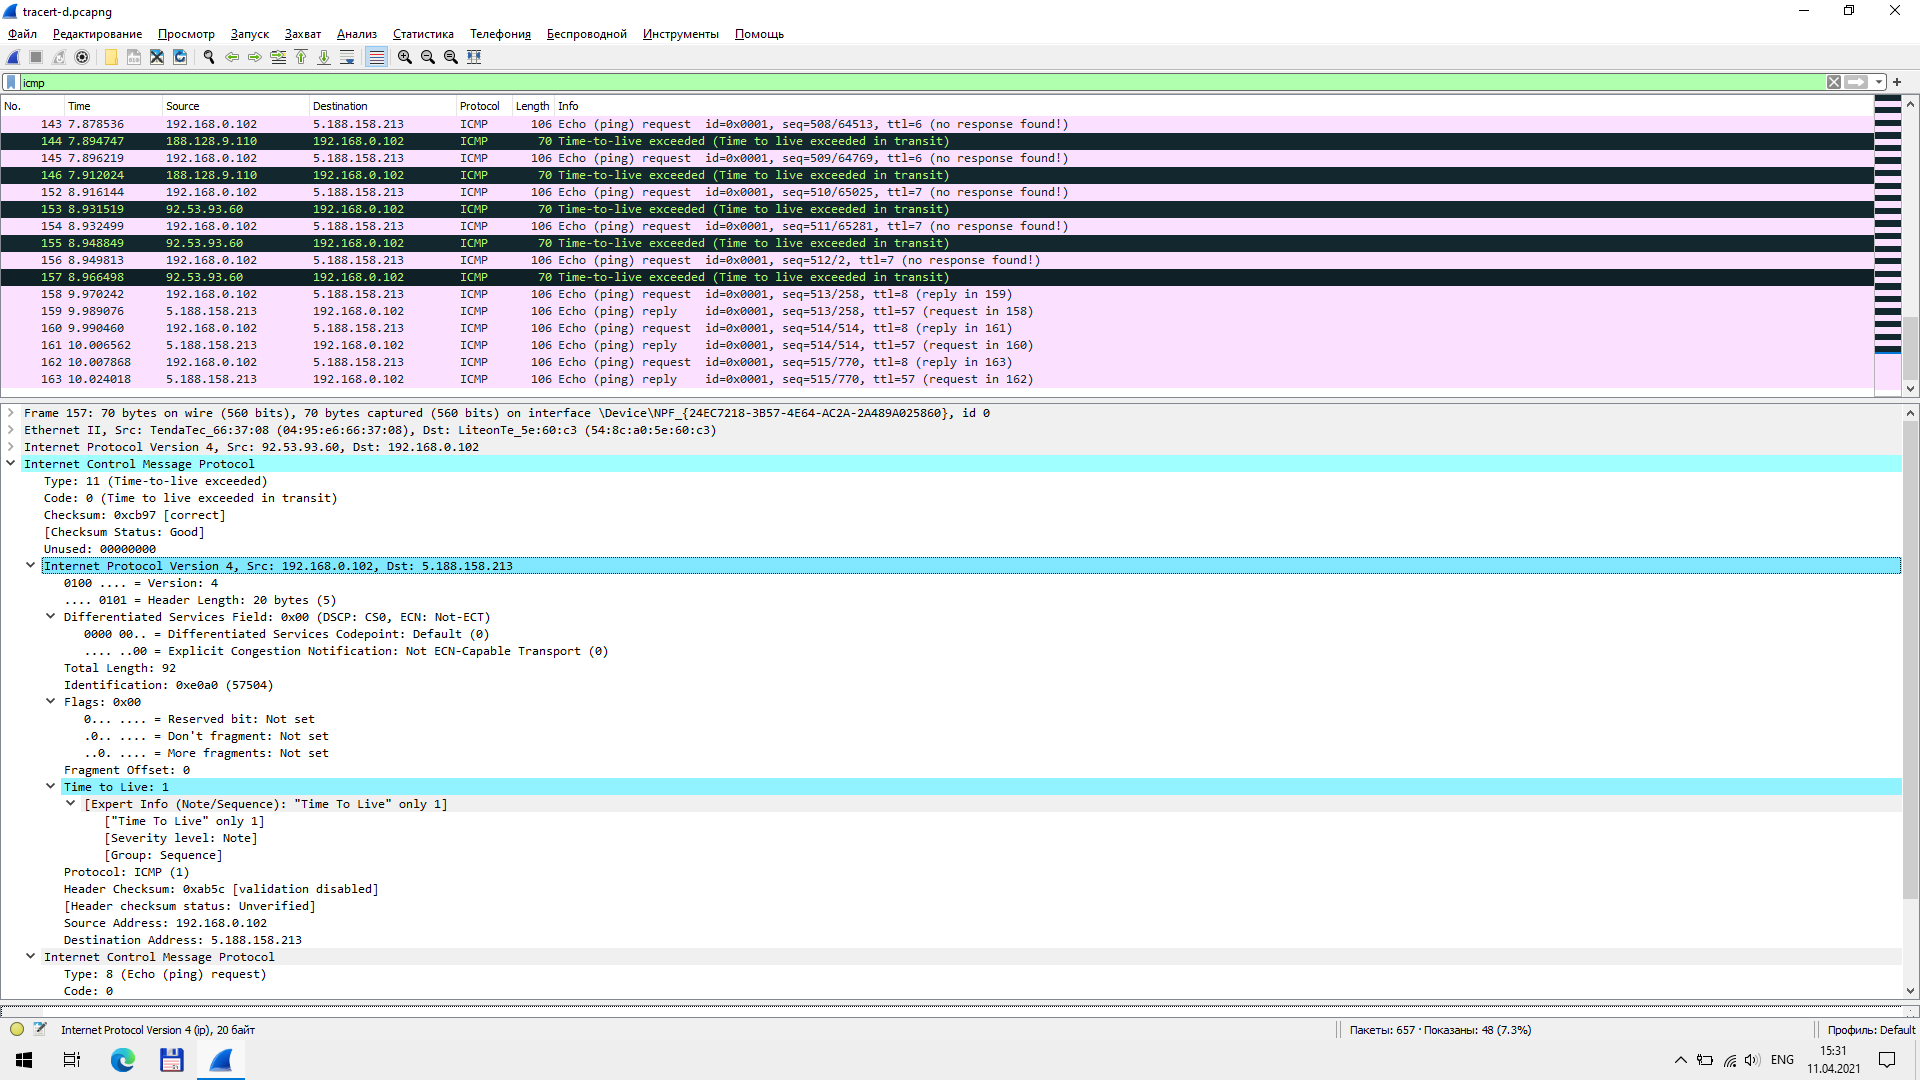
\includegraphics[width=\textwidth]{screenshots/tracert-d_ttl_response_2}

    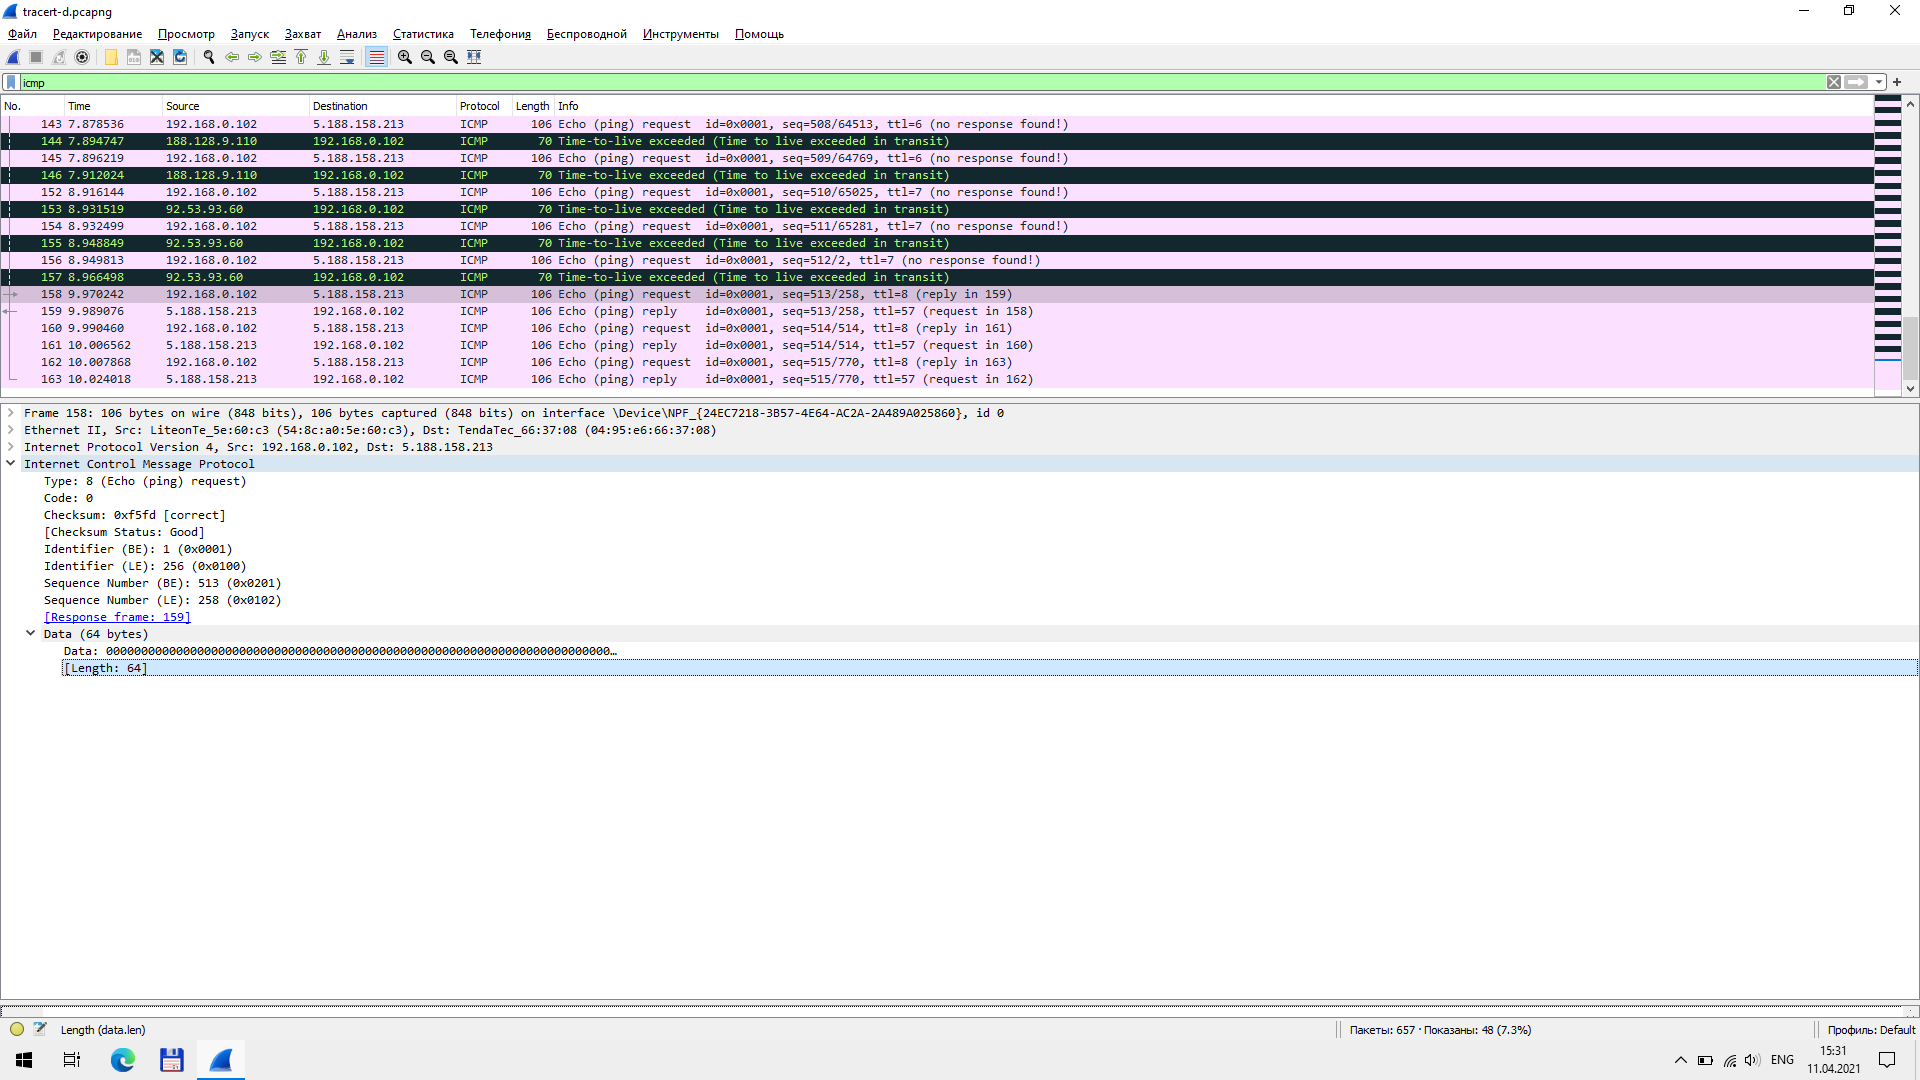
\includegraphics[width=\textwidth]{screenshots/tracert-d_success_request_1}

    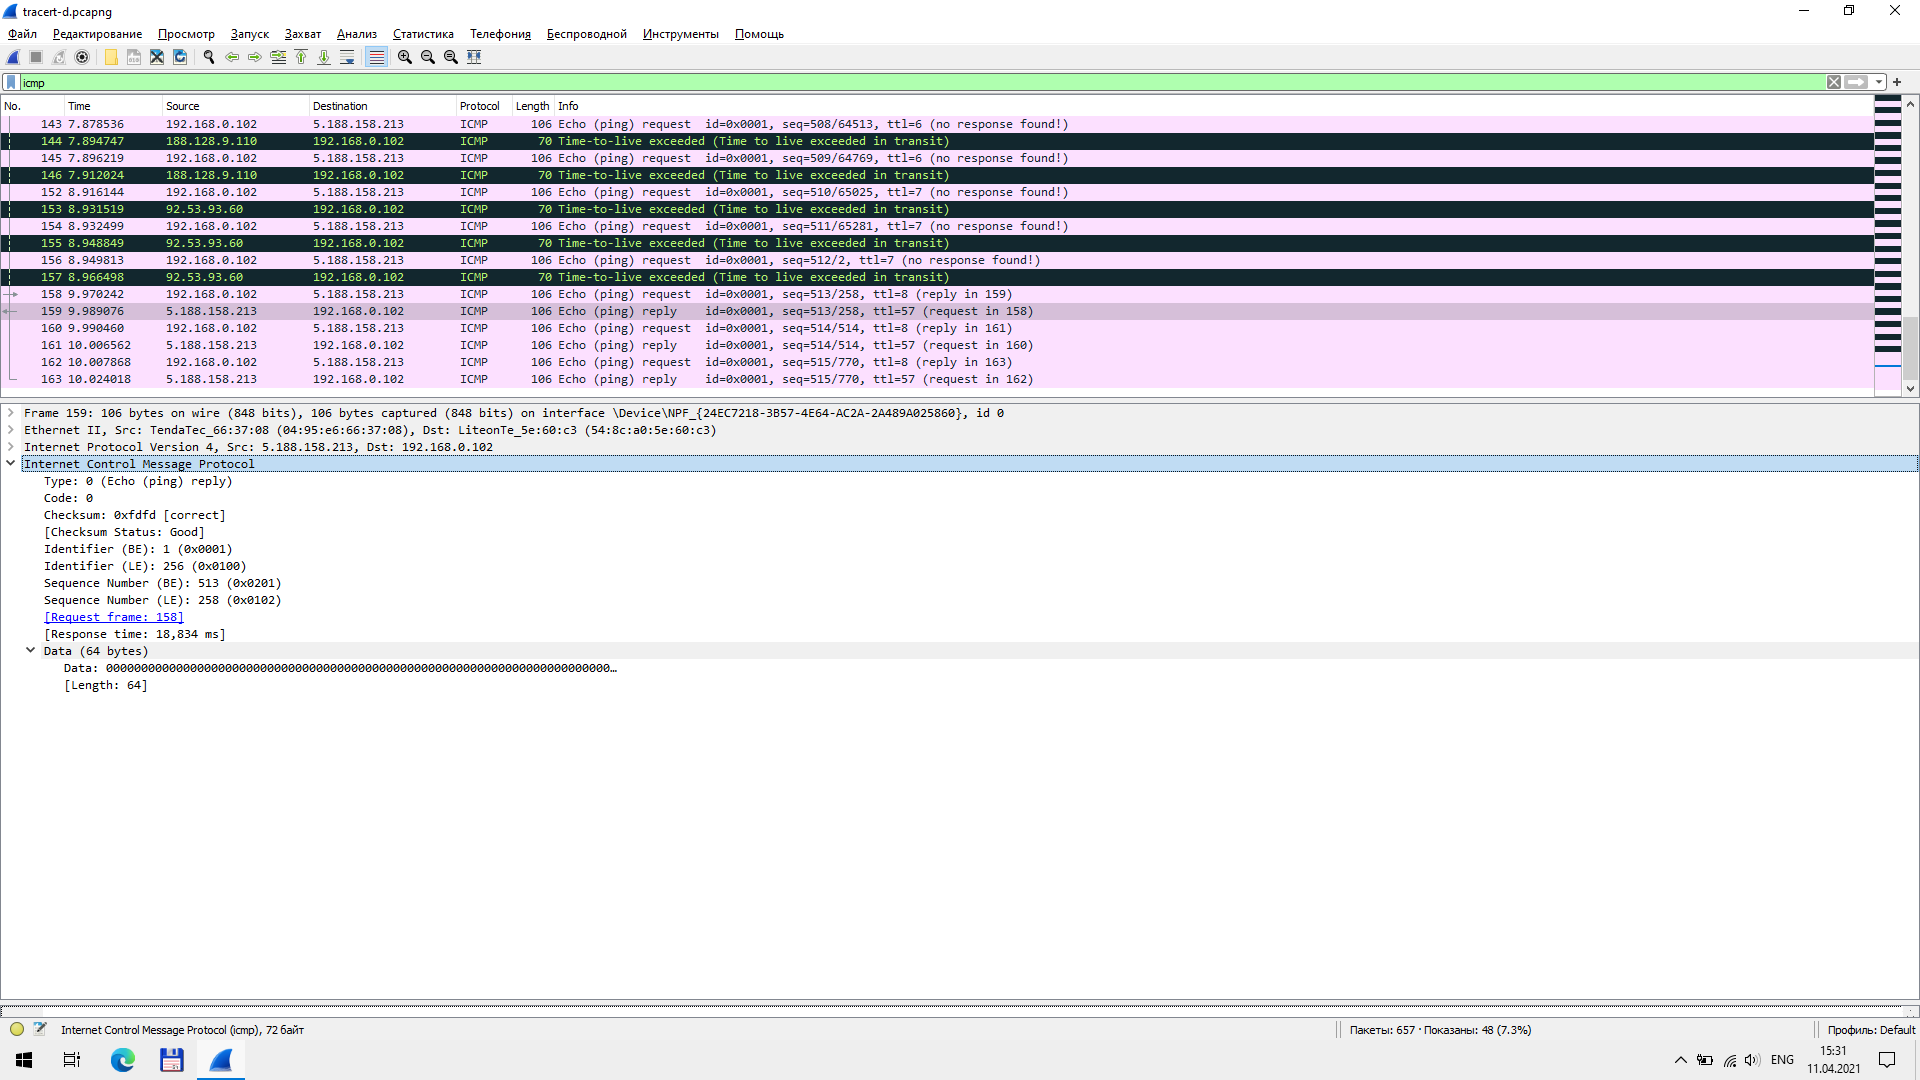
\includegraphics[width=\textwidth]{screenshots/tracert-d_success_response_1}

    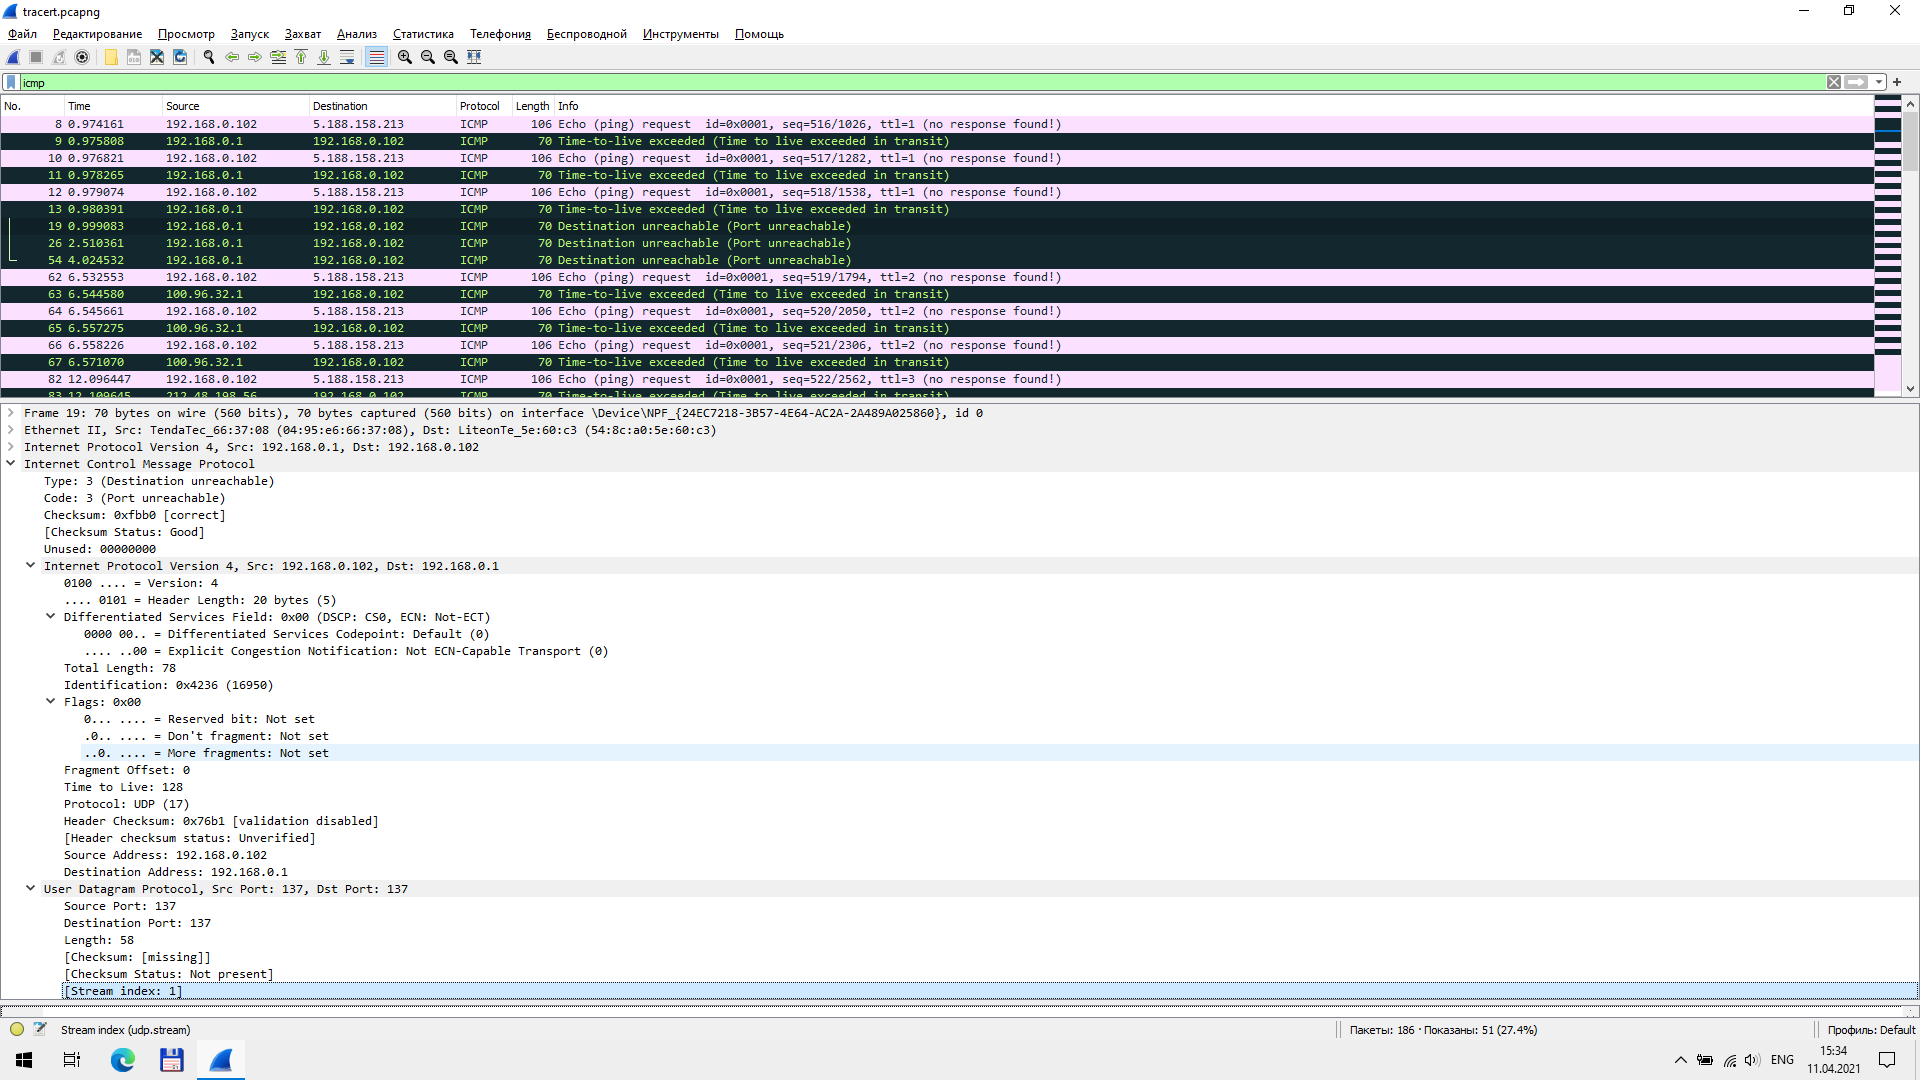
\includegraphics[width=\textwidth]{screenshots/tracert_port_1}

    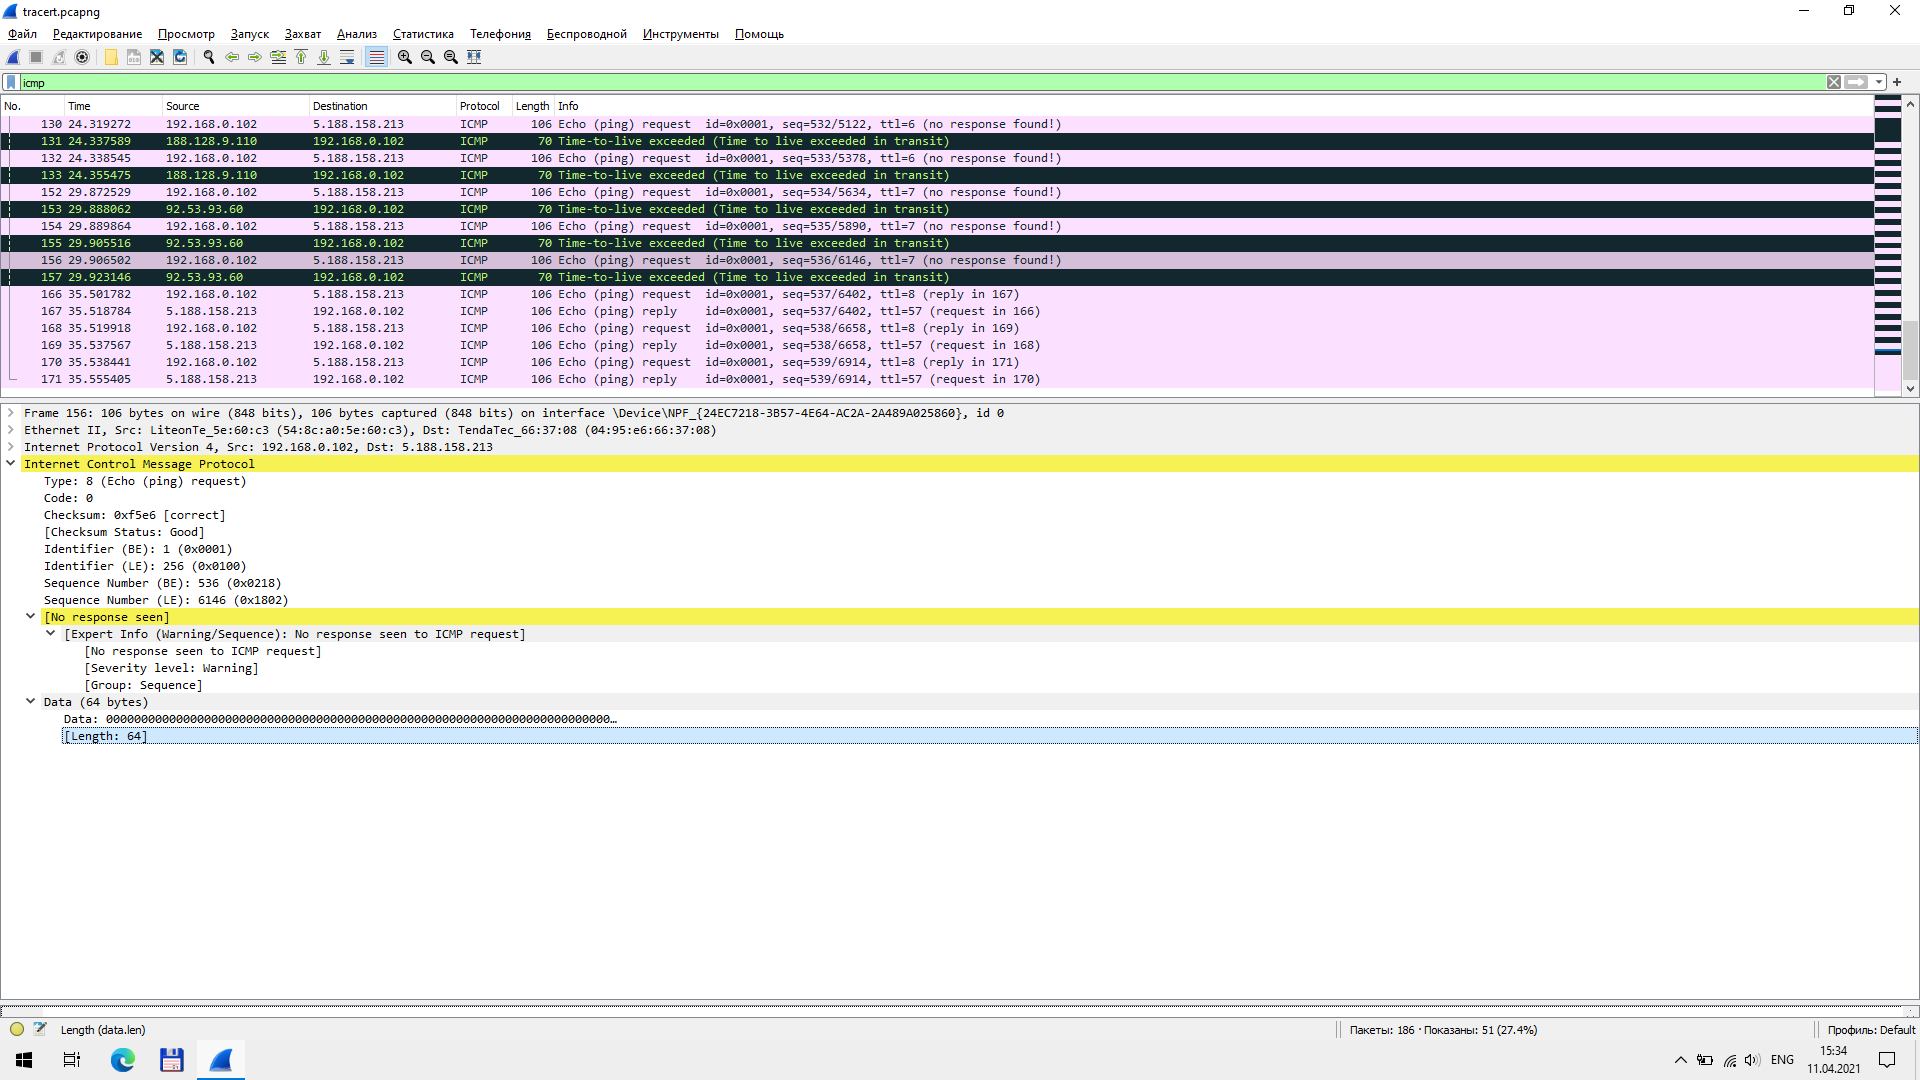
\includegraphics[width=\textwidth]{screenshots/tracert_ttl_request_1}

    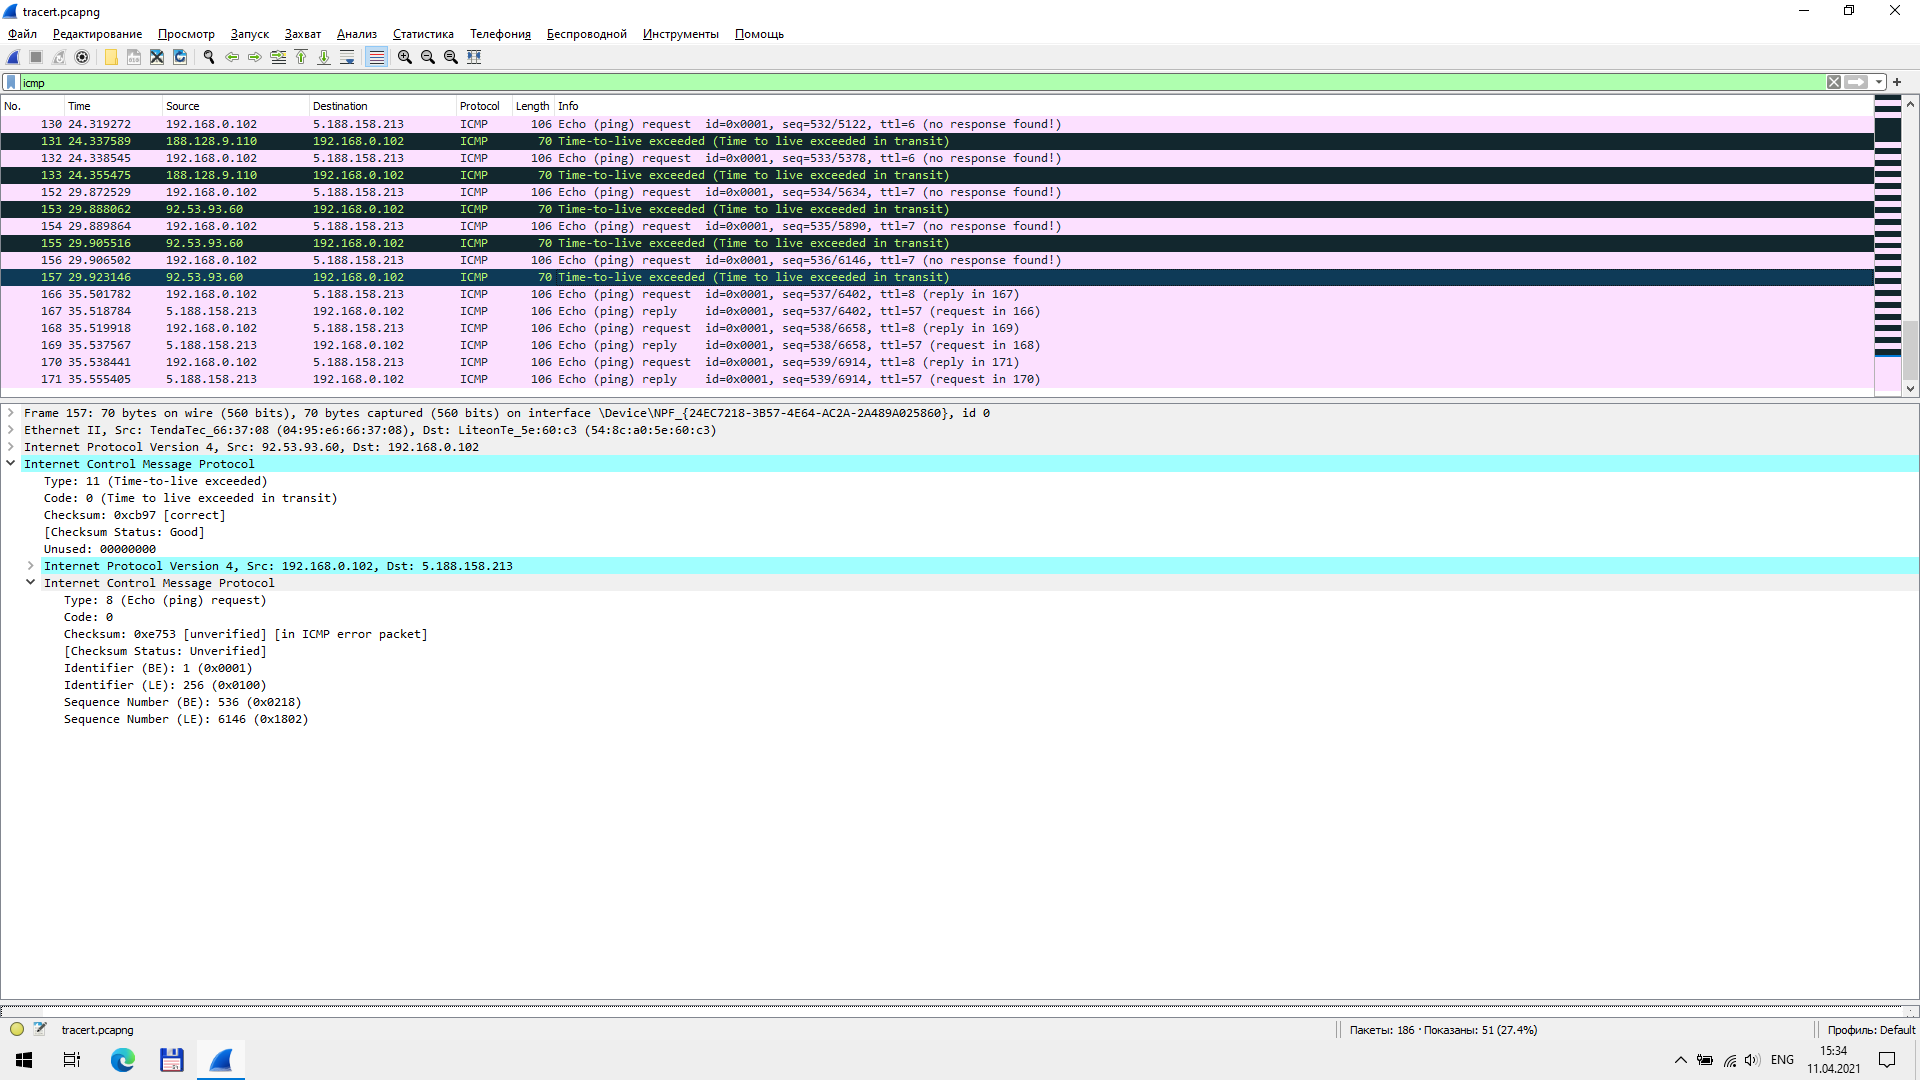
\includegraphics[width=\textwidth]{screenshots/tracert_ttl_response_1}

    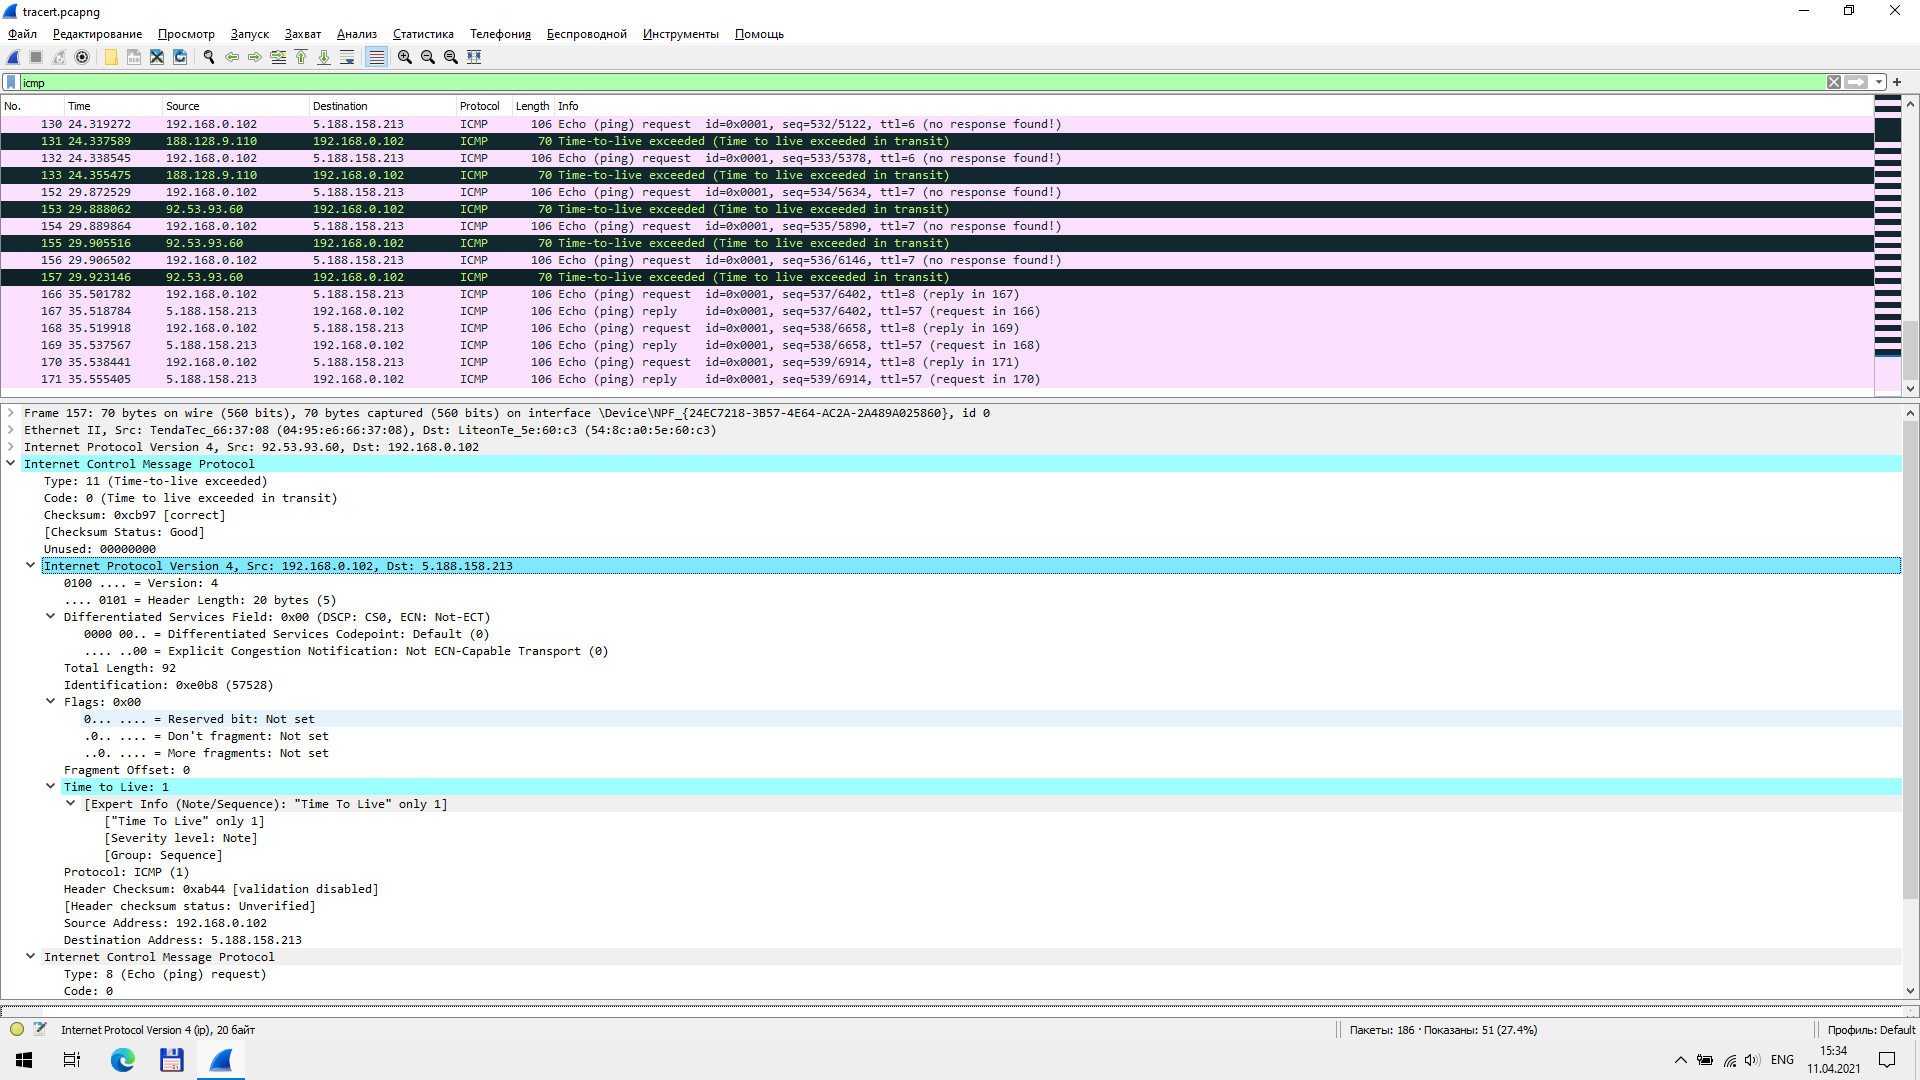
\includegraphics[width=\textwidth]{screenshots/tracert_ttl_response_2}

    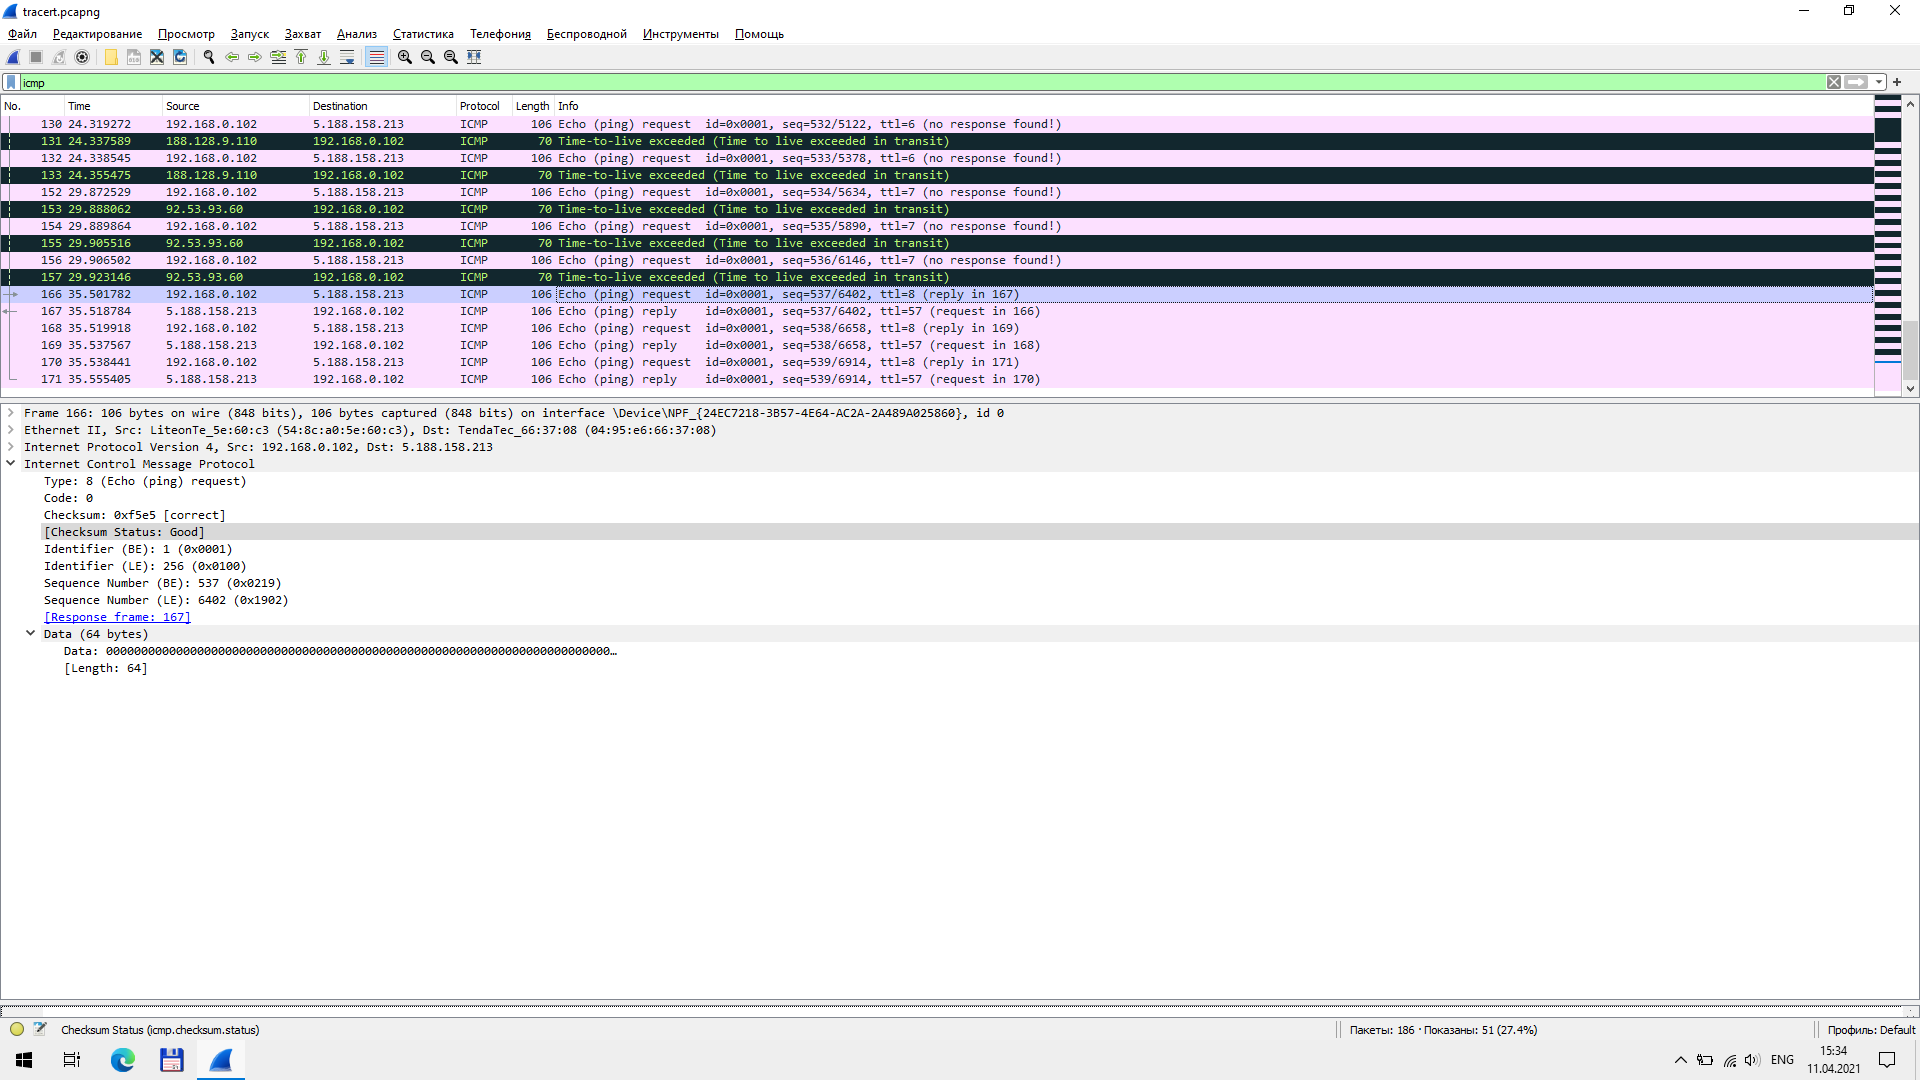
\includegraphics[width=\textwidth]{screenshots/tracert_success_request_1}

    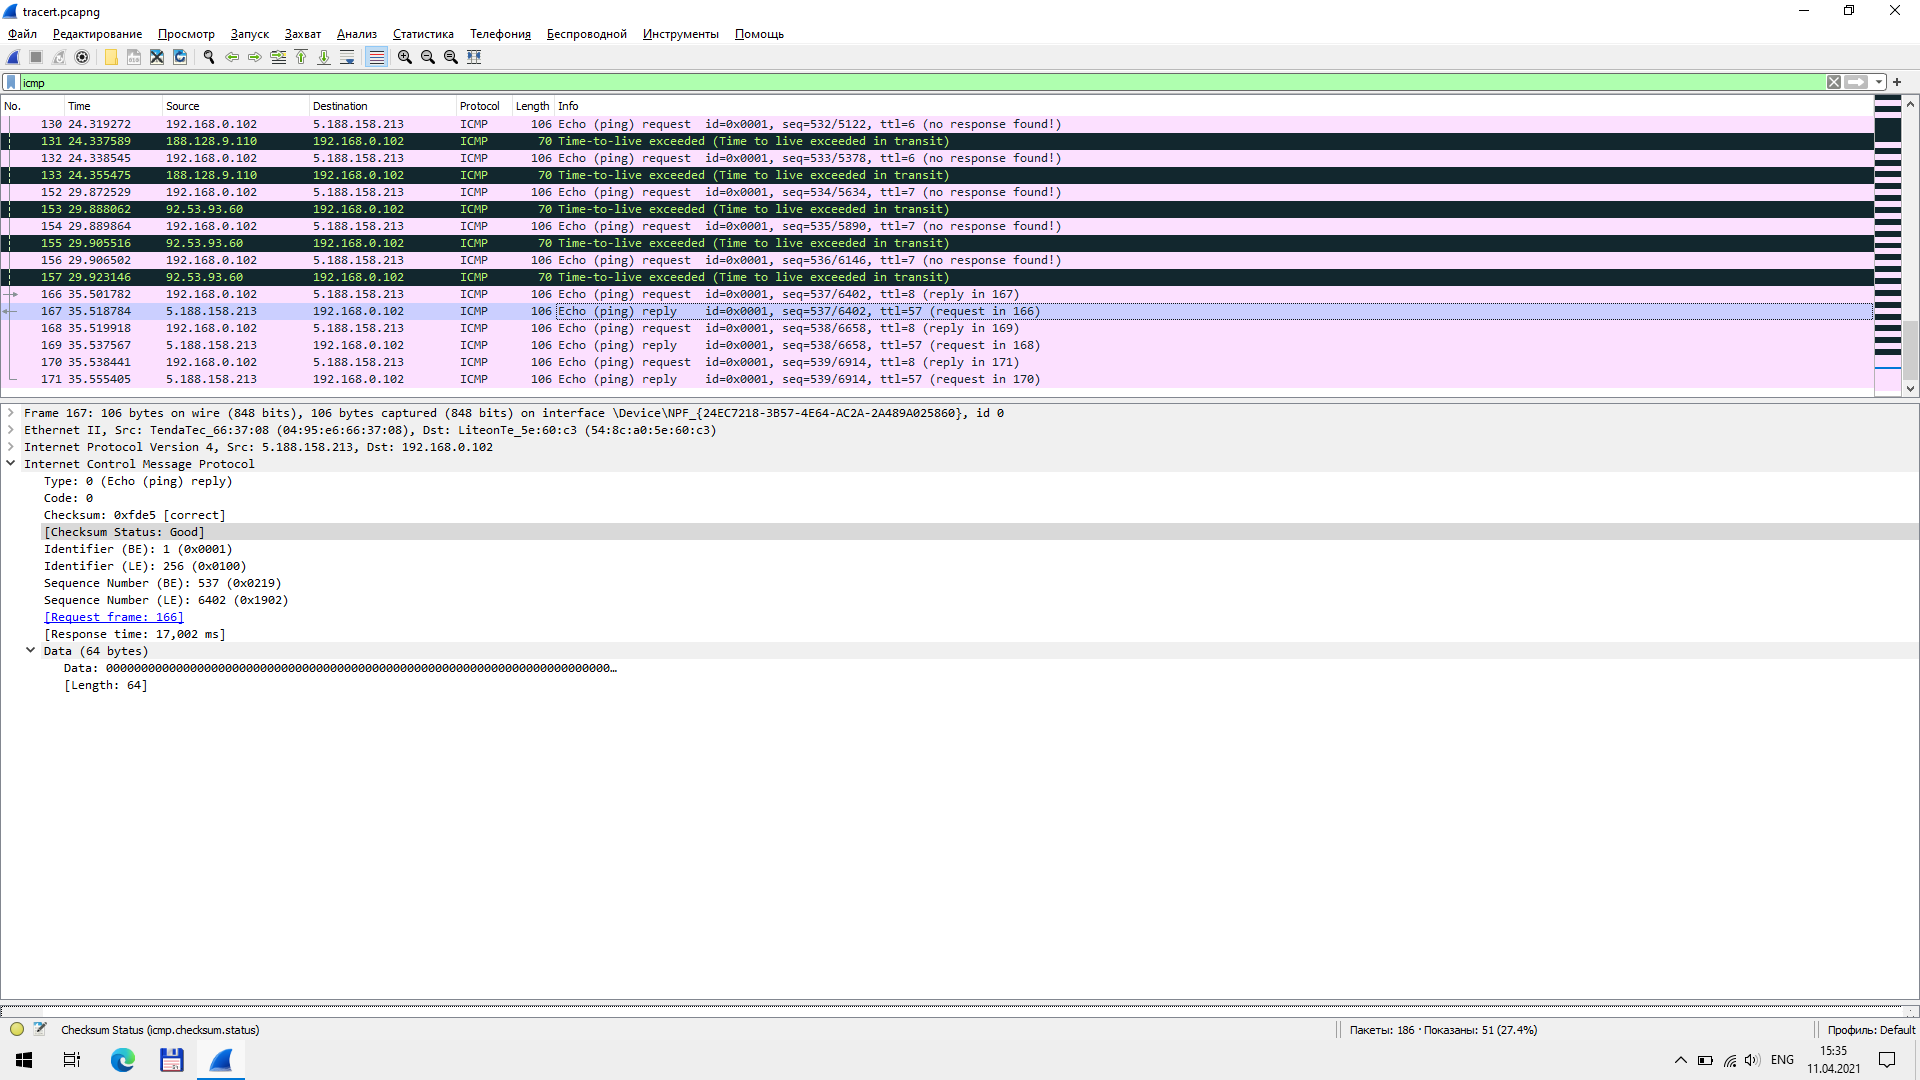
\includegraphics[width=\textwidth]{screenshots/tracert_success_response_1}

\end{center}

\subsection{Ответы на вопросы}

\subsubsection{}
20 байт (согласно анализу Wireshark).
Поле данных --- 72 байта для tracert, до 1480 байт в общем случае.

\subsubsection{}
Каждая пересылка уменьшает TTL на 1.
Если TTL достиг 1, то посылается обратное сообщение с TTL=255 о том, что TTL исчерпан.

\subsubsection{}
IP-фреймы tracert увеличивают TTL с каждой итерацией, а ICMP содержат нули в поле данных.

\subsubsection{}
Полем Type в заголовке ICMP, а ошибочные ответы также содержат информацию о провалившемся запросе в поле данных.

\subsubsection{}
Без ключа \texttt{-d} утилита \texttt{tracert} будет также запрашивать имена промежуточных узлов (есть не у всех).
